\documentclass[twoside]{book}

% Packages required by doxygen
\usepackage{fixltx2e}
\usepackage{calc}
\usepackage{doxygen}
\usepackage[export]{adjustbox} % also loads graphicx
\usepackage{graphicx}
\usepackage[utf8]{inputenc}
\usepackage{makeidx}
\usepackage{multicol}
\usepackage{multirow}
\PassOptionsToPackage{warn}{textcomp}
\usepackage{textcomp}
\usepackage[nointegrals]{wasysym}
\usepackage[table]{xcolor}

% Font selection
\usepackage[T1]{fontenc}
\usepackage[scaled=.90]{helvet}
\usepackage{courier}
\usepackage{amssymb}
\usepackage{sectsty}
\renewcommand{\familydefault}{\sfdefault}
\allsectionsfont{%
  \fontseries{bc}\selectfont%
  \color{darkgray}%
}
\renewcommand{\DoxyLabelFont}{%
  \fontseries{bc}\selectfont%
  \color{darkgray}%
}
\newcommand{\+}{\discretionary{\mbox{\scriptsize$\hookleftarrow$}}{}{}}

% Page & text layout
\usepackage{geometry}
\geometry{%
  a4paper,%
  top=2.5cm,%
  bottom=2.5cm,%
  left=2.5cm,%
  right=2.5cm%
}
\tolerance=750
\hfuzz=15pt
\hbadness=750
\setlength{\emergencystretch}{15pt}
\setlength{\parindent}{0cm}
\setlength{\parskip}{3ex plus 2ex minus 2ex}
\makeatletter
\renewcommand{\paragraph}{%
  \@startsection{paragraph}{4}{0ex}{-1.0ex}{1.0ex}{%
    \normalfont\normalsize\bfseries\SS@parafont%
  }%
}
\renewcommand{\subparagraph}{%
  \@startsection{subparagraph}{5}{0ex}{-1.0ex}{1.0ex}{%
    \normalfont\normalsize\bfseries\SS@subparafont%
  }%
}
\makeatother

% Headers & footers
\usepackage{fancyhdr}
\pagestyle{fancyplain}
\fancyhead[LE]{\fancyplain{}{\bfseries\thepage}}
\fancyhead[CE]{\fancyplain{}{}}
\fancyhead[RE]{\fancyplain{}{\bfseries\leftmark}}
\fancyhead[LO]{\fancyplain{}{\bfseries\rightmark}}
\fancyhead[CO]{\fancyplain{}{}}
\fancyhead[RO]{\fancyplain{}{\bfseries\thepage}}
\fancyfoot[LE]{\fancyplain{}{}}
\fancyfoot[CE]{\fancyplain{}{}}
\fancyfoot[RE]{\fancyplain{}{\bfseries\scriptsize Generated by Doxygen }}
\fancyfoot[LO]{\fancyplain{}{\bfseries\scriptsize Generated by Doxygen }}
\fancyfoot[CO]{\fancyplain{}{}}
\fancyfoot[RO]{\fancyplain{}{}}
\renewcommand{\footrulewidth}{0.4pt}
\renewcommand{\chaptermark}[1]{%
  \markboth{#1}{}%
}
\renewcommand{\sectionmark}[1]{%
  \markright{\thesection\ #1}%
}

% Indices & bibliography
\usepackage{natbib}
\usepackage[titles]{tocloft}
\setcounter{tocdepth}{3}
\setcounter{secnumdepth}{5}
\makeindex

% Hyperlinks (required, but should be loaded last)
\usepackage{ifpdf}
\ifpdf
  \usepackage[pdftex,pagebackref=true]{hyperref}
\else
  \usepackage[ps2pdf,pagebackref=true]{hyperref}
\fi
\hypersetup{%
  colorlinks=true,%
  linkcolor=blue,%
  citecolor=blue,%
  unicode%
}

% Custom commands
\newcommand{\clearemptydoublepage}{%
  \newpage{\pagestyle{empty}\cleardoublepage}%
}

\usepackage{caption}
\captionsetup{labelsep=space,justification=centering,font={bf},singlelinecheck=off,skip=4pt,position=top}

%===== C O N T E N T S =====

\begin{document}

% Titlepage & ToC
\hypersetup{pageanchor=false,
             bookmarksnumbered=true,
             pdfencoding=unicode
            }
\pagenumbering{alph}
\begin{titlepage}
\vspace*{7cm}
\begin{center}%
{\Large Treadmill Automation }\\
\vspace*{1cm}
{\large Generated by Doxygen 1.8.13}\\
\end{center}
\end{titlepage}
\clearemptydoublepage
\pagenumbering{roman}
\tableofcontents
\clearemptydoublepage
\pagenumbering{arabic}
\hypersetup{pageanchor=true}

%--- Begin generated contents ---
\chapter{File Index}
\section{File List}
Here is a list of all files with brief descriptions\+:\begin{DoxyCompactList}
\item\contentsline{section}{src/\hyperlink{_config_tab_widget_8cpp}{Config\+Tab\+Widget.\+cpp} }{\pageref{_config_tab_widget_8cpp}}{}
\item\contentsline{section}{src/\hyperlink{_data_collection_8cpp}{Data\+Collection.\+cpp} }{\pageref{_data_collection_8cpp}}{}
\item\contentsline{section}{src/\hyperlink{_data_source_8cpp}{Data\+Source.\+cpp} }{\pageref{_data_source_8cpp}}{}
\item\contentsline{section}{src/\hyperlink{_instrumentation_panel_8cpp}{Instrumentation\+Panel.\+cpp} }{\pageref{_instrumentation_panel_8cpp}}{}
\item\contentsline{section}{src/\hyperlink{main_8cpp}{main.\+cpp} }{\pageref{main_8cpp}}{}
\item\contentsline{section}{src/\hyperlink{_manage_profile_tab_widget_8cpp}{Manage\+Profile\+Tab\+Widget.\+cpp} }{\pageref{_manage_profile_tab_widget_8cpp}}{}
\item\contentsline{section}{src/\hyperlink{_mcc_daq_connect_button_widget_8cpp}{Mcc\+Daq\+Connect\+Button\+Widget.\+cpp} }{\pageref{_mcc_daq_connect_button_widget_8cpp}}{}
\item\contentsline{section}{src/\hyperlink{_mcc_daq_discovery_8cpp}{Mcc\+Daq\+Discovery.\+cpp} }{\pageref{_mcc_daq_discovery_8cpp}}{}
\item\contentsline{section}{src/\hyperlink{_mcc_daq_interface_8cpp}{Mcc\+Daq\+Interface.\+cpp} }{\pageref{_mcc_daq_interface_8cpp}}{}
\item\contentsline{section}{src/\hyperlink{_mcc_daq_record_button_widget_8cpp}{Mcc\+Daq\+Record\+Button\+Widget.\+cpp} }{\pageref{_mcc_daq_record_button_widget_8cpp}}{}
\item\contentsline{section}{src/\hyperlink{_mouse_interface_8cpp}{Mouse\+Interface.\+cpp} }{\pageref{_mouse_interface_8cpp}}{}
\item\contentsline{section}{src/\hyperlink{_network_tab_widget_8cpp}{Network\+Tab\+Widget.\+cpp} }{\pageref{_network_tab_widget_8cpp}}{}
\item\contentsline{section}{src/\hyperlink{_network_tab_widget_lights_8cpp}{Network\+Tab\+Widget\+Lights.\+cpp} }{\pageref{_network_tab_widget_lights_8cpp}}{}
\item\contentsline{section}{src/\hyperlink{_parse_run_profile_8cpp}{Parse\+Run\+Profile.\+cpp} }{\pageref{_parse_run_profile_8cpp}}{}
\item\contentsline{section}{src/\hyperlink{_perturbation_tab_widget_8cpp}{Perturbation\+Tab\+Widget.\+cpp} }{\pageref{_perturbation_tab_widget_8cpp}}{}
\item\contentsline{section}{src/\hyperlink{_qml_interface_8cpp}{Qml\+Interface.\+cpp} }{\pageref{_qml_interface_8cpp}}{}
\item\contentsline{section}{src/\hyperlink{_read_trial_name_file_8cpp}{Read\+Trial\+Name\+File.\+cpp} }{\pageref{_read_trial_name_file_8cpp}}{}
\item\contentsline{section}{src/\hyperlink{_record_treadmill_stream_8cpp}{Record\+Treadmill\+Stream.\+cpp} }{\pageref{_record_treadmill_stream_8cpp}}{}
\item\contentsline{section}{src/\hyperlink{_send_setpoints_8cpp}{Send\+Setpoints.\+cpp} }{\pageref{_send_setpoints_8cpp}}{}
\item\contentsline{section}{src/\hyperlink{_stimulator_interface_8cpp}{Stimulator\+Interface.\+cpp} }{\pageref{_stimulator_interface_8cpp}}{}
\item\contentsline{section}{src/\hyperlink{_subject_interface_8cpp}{Subject\+Interface.\+cpp} }{\pageref{_subject_interface_8cpp}}{}
\item\contentsline{section}{src/\hyperlink{_subject_interface_widget_8cpp}{Subject\+Interface\+Widget.\+cpp} }{\pageref{_subject_interface_widget_8cpp}}{}
\item\contentsline{section}{src/\hyperlink{_treadmill_automation_8cpp}{Treadmill\+Automation.\+cpp} }{\pageref{_treadmill_automation_8cpp}}{}
\item\contentsline{section}{src/\hyperlink{_treadmill_automation_db_i_face_8cpp}{Treadmill\+Automation\+Db\+I\+Face.\+cpp} }{\pageref{_treadmill_automation_db_i_face_8cpp}}{}
\end{DoxyCompactList}

\chapter{File Documentation}
\hypertarget{_config_tab_widget_8cpp}{}\section{src/\+Config\+Tab\+Widget.cpp File Reference}
\label{_config_tab_widget_8cpp}\index{src/\+Config\+Tab\+Widget.\+cpp@{src/\+Config\+Tab\+Widget.\+cpp}}
{\ttfamily \#include \char`\"{}Config\+Tab\+Widget.\+h\char`\"{}}\newline
{\ttfamily \#include \char`\"{}../include/moc\+\_\+\+Config\+Tab\+Widget.\+cpp\char`\"{}}\newline
Include dependency graph for Config\+Tab\+Widget.\+cpp\+:
\nopagebreak
\begin{figure}[H]
\begin{center}
\leavevmode
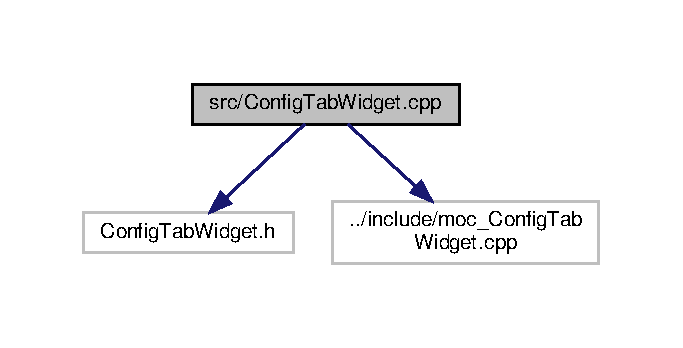
\includegraphics[width=328pt]{_config_tab_widget_8cpp__incl}
\end{center}
\end{figure}

\hypertarget{_data_collection_8cpp}{}\section{src/\+Data\+Collection.cpp File Reference}
\label{_data_collection_8cpp}\index{src/\+Data\+Collection.\+cpp@{src/\+Data\+Collection.\+cpp}}
{\ttfamily \#include \char`\"{}Data\+Collection.\+h\char`\"{}}\newline
{\ttfamily \#include \char`\"{}../include/moc\+\_\+\+Data\+Collection.\+cpp\char`\"{}}\newline
Include dependency graph for Data\+Collection.\+cpp\+:
\nopagebreak
\begin{figure}[H]
\begin{center}
\leavevmode
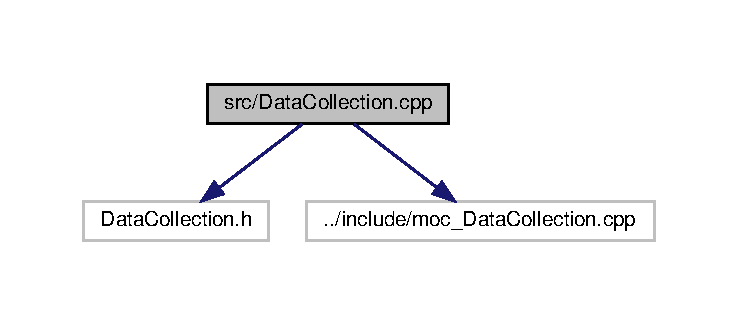
\includegraphics[width=350pt]{_data_collection_8cpp__incl}
\end{center}
\end{figure}

\hypertarget{_data_source_8cpp}{}\section{src/\+Data\+Source.cpp File Reference}
\label{_data_source_8cpp}\index{src/\+Data\+Source.\+cpp@{src/\+Data\+Source.\+cpp}}
{\ttfamily \#include \char`\"{}Datasource.\+h\char`\"{}}\newline
{\ttfamily \#include $<$Qt\+Charts/\+Q\+X\+Y\+Series$>$}\newline
{\ttfamily \#include $<$Qt\+Charts/\+Q\+Area\+Series$>$}\newline
{\ttfamily \#include $<$Qt\+Quick/\+Q\+Quick\+View$>$}\newline
{\ttfamily \#include $<$Qt\+Quick/\+Q\+Quick\+Item$>$}\newline
{\ttfamily \#include $<$Qt\+Core/\+Q\+Debug$>$}\newline
{\ttfamily \#include $<$Qt\+Core/\+Q\+Random\+Generator$>$}\newline
{\ttfamily \#include $<$Qt\+Core/\+Qt\+Math$>$}\newline
{\ttfamily \#include \char`\"{}../include/moc\+\_\+\+Data\+Source.\+cpp\char`\"{}}\newline
Include dependency graph for Data\+Source.\+cpp\+:
\nopagebreak
\begin{figure}[H]
\begin{center}
\leavevmode
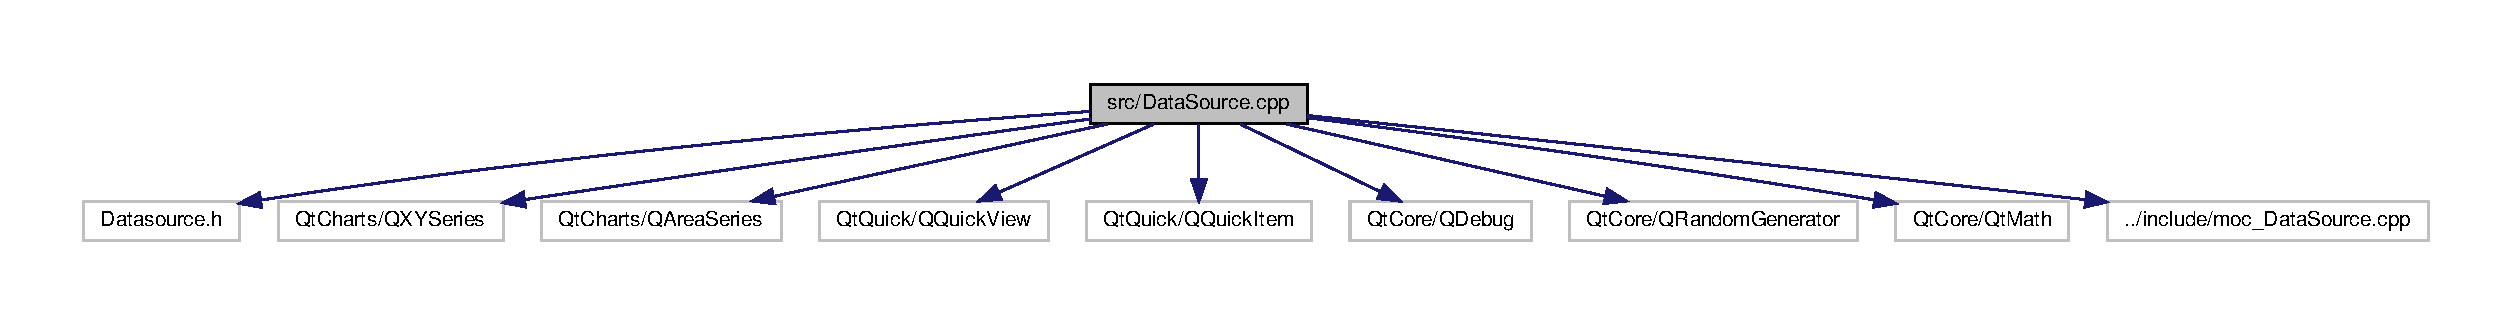
\includegraphics[width=350pt]{_data_source_8cpp__incl}
\end{center}
\end{figure}

\hypertarget{_instrumentation_panel_8cpp}{}\section{src/\+Instrumentation\+Panel.cpp File Reference}
\label{_instrumentation_panel_8cpp}\index{src/\+Instrumentation\+Panel.\+cpp@{src/\+Instrumentation\+Panel.\+cpp}}
{\ttfamily \#include \char`\"{}../include/\+Instrumentation\+Panel.\+h\char`\"{}}\newline
{\ttfamily \#include \char`\"{}../include/moc\+\_\+\+Instrumentation\+Panel.\+cpp\char`\"{}}\newline
Include dependency graph for Instrumentation\+Panel.\+cpp\+:
\nopagebreak
\begin{figure}[H]
\begin{center}
\leavevmode
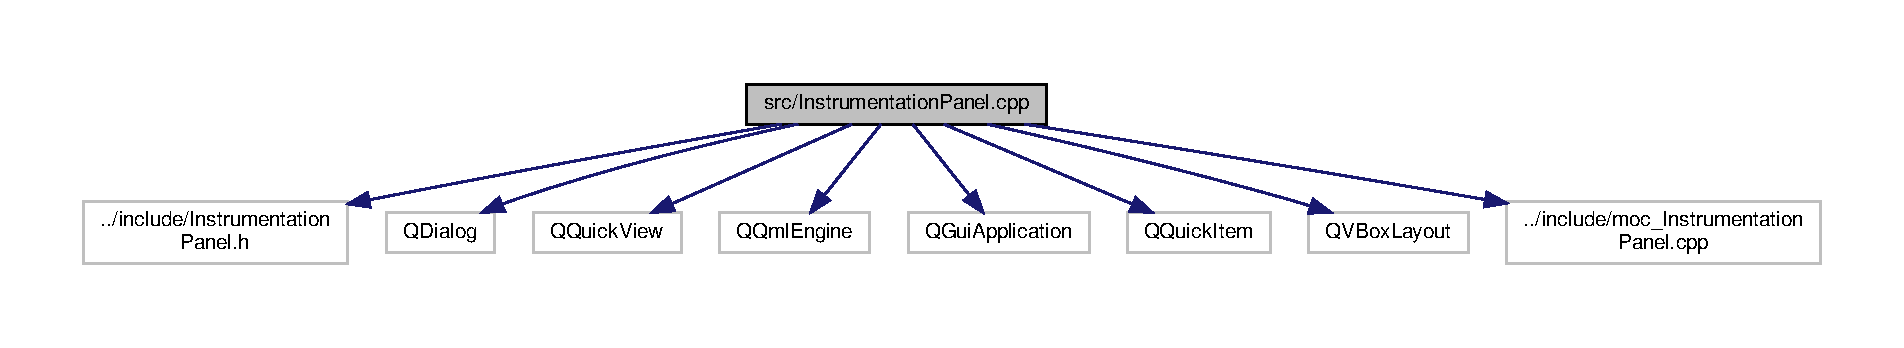
\includegraphics[width=350pt]{_instrumentation_panel_8cpp__incl}
\end{center}
\end{figure}

\hypertarget{main_8cpp}{}\section{src/main.cpp File Reference}
\label{main_8cpp}\index{src/main.\+cpp@{src/main.\+cpp}}
{\ttfamily \#include \char`\"{}include/\+Treadmill\+Automation.\+h\char`\"{}}\newline
{\ttfamily \#include $<$Qt\+Widgets/\+Q\+Application$>$}\newline
{\ttfamily \#include $<$Q\+Scoped\+Pointer$>$}\newline
Include dependency graph for main.\+cpp\+:
\nopagebreak
\begin{figure}[H]
\begin{center}
\leavevmode
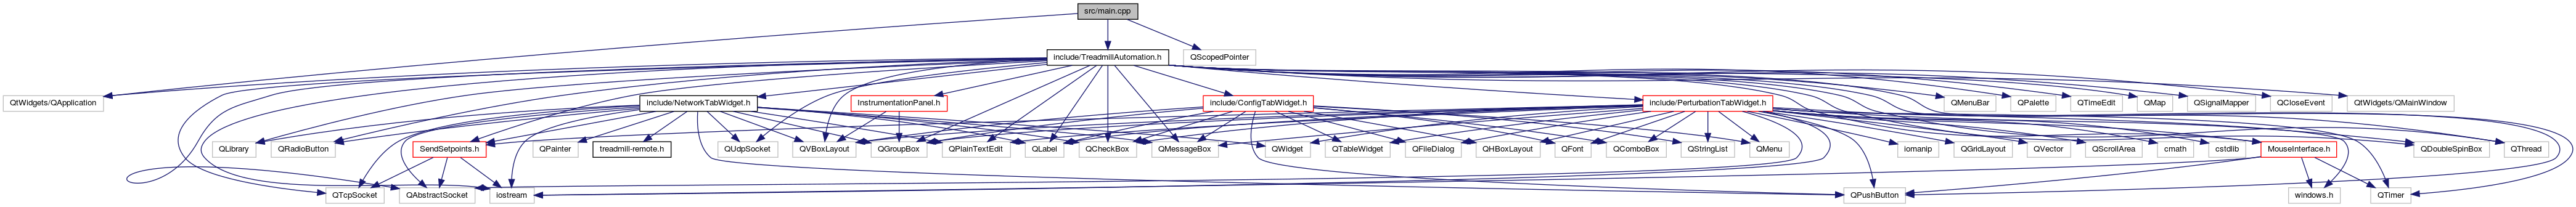
\includegraphics[width=350pt]{main_8cpp__incl}
\end{center}
\end{figure}
\subsection*{Functions}
\begin{DoxyCompactItemize}
\item 
int \hyperlink{main_8cpp_a0ddf1224851353fc92bfbff6f499fa97}{main} (int argc, char $\ast$argv\mbox{[}$\,$\mbox{]})
\end{DoxyCompactItemize}


\subsection{Function Documentation}
\mbox{\Hypertarget{main_8cpp_a0ddf1224851353fc92bfbff6f499fa97}\label{main_8cpp_a0ddf1224851353fc92bfbff6f499fa97}} 
\index{main.\+cpp@{main.\+cpp}!main@{main}}
\index{main@{main}!main.\+cpp@{main.\+cpp}}
\subsubsection{\texorpdfstring{main()}{main()}}
{\footnotesize\ttfamily int main (\begin{DoxyParamCaption}\item[{int}]{argc,  }\item[{char $\ast$}]{argv\mbox{[}$\,$\mbox{]} }\end{DoxyParamCaption})}



Definition at line 5 of file main.\+cpp.


\hypertarget{_manage_profile_tab_widget_8cpp}{}\section{src/\+Manage\+Profile\+Tab\+Widget.cpp File Reference}
\label{_manage_profile_tab_widget_8cpp}\index{src/\+Manage\+Profile\+Tab\+Widget.\+cpp@{src/\+Manage\+Profile\+Tab\+Widget.\+cpp}}
{\ttfamily \#include \char`\"{}../include/\+Manage\+Profile\+Tab\+Widget.\+h\char`\"{}}\newline
{\ttfamily \#include \char`\"{}../include/moc\+\_\+\+Manage\+Profile\+Tab\+Widget.\+cpp\char`\"{}}\newline
Include dependency graph for Manage\+Profile\+Tab\+Widget.\+cpp\+:
\nopagebreak
\begin{figure}[H]
\begin{center}
\leavevmode
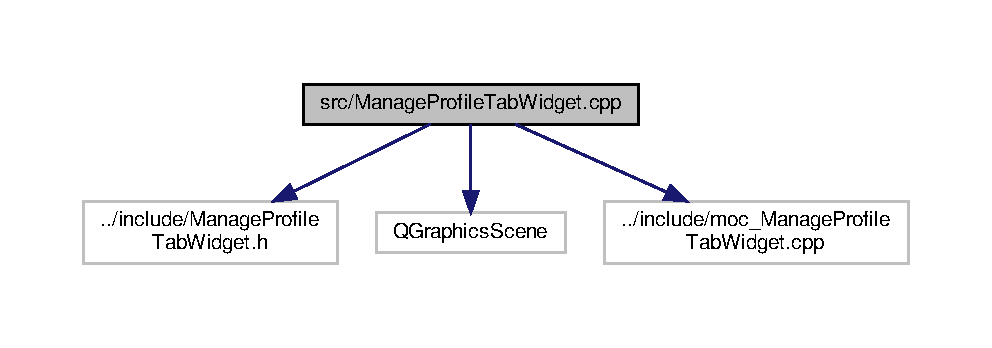
\includegraphics[width=350pt]{_manage_profile_tab_widget_8cpp__incl}
\end{center}
\end{figure}

\hypertarget{_mcc_daq_connect_button_widget_8cpp}{}\section{src/\+Mcc\+Daq\+Connect\+Button\+Widget.cpp File Reference}
\label{_mcc_daq_connect_button_widget_8cpp}\index{src/\+Mcc\+Daq\+Connect\+Button\+Widget.\+cpp@{src/\+Mcc\+Daq\+Connect\+Button\+Widget.\+cpp}}
{\ttfamily \#include \char`\"{}Mcc\+Daq\+Connect\+Button\+Widget.\+h\char`\"{}}\newline
{\ttfamily \#include \char`\"{}../include/moc\+\_\+\+Mcc\+Daq\+Connect\+Button\+Widget.\+cpp\char`\"{}}\newline
Include dependency graph for Mcc\+Daq\+Connect\+Button\+Widget.\+cpp\+:
\nopagebreak
\begin{figure}[H]
\begin{center}
\leavevmode
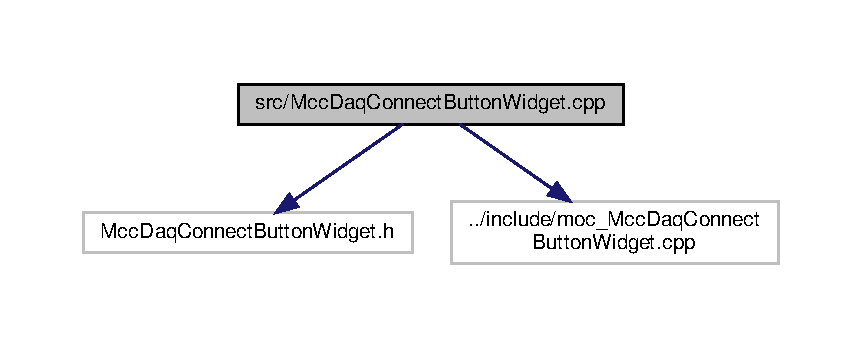
\includegraphics[width=350pt]{_mcc_daq_connect_button_widget_8cpp__incl}
\end{center}
\end{figure}

\hypertarget{_mcc_daq_discovery_8cpp}{}\section{src/\+Mcc\+Daq\+Discovery.cpp File Reference}
\label{_mcc_daq_discovery_8cpp}\index{src/\+Mcc\+Daq\+Discovery.\+cpp@{src/\+Mcc\+Daq\+Discovery.\+cpp}}
{\ttfamily \#include \char`\"{}Mcc\+Daq\+Discovery.\+h\char`\"{}}\newline
{\ttfamily \#include \char`\"{}../include/moc\+\_\+\+Mcc\+Daq\+Discovery.\+cpp\char`\"{}}\newline
Include dependency graph for Mcc\+Daq\+Discovery.\+cpp\+:
\nopagebreak
\begin{figure}[H]
\begin{center}
\leavevmode
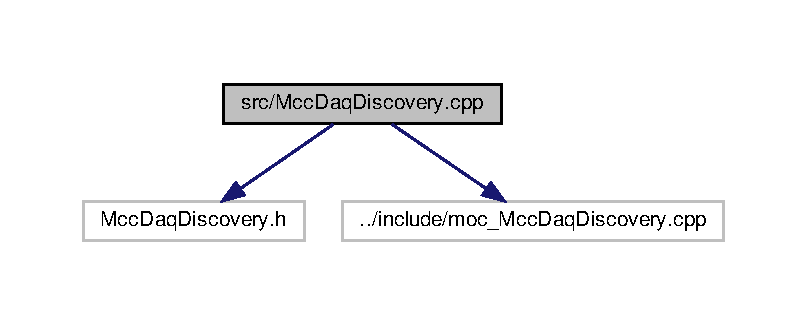
\includegraphics[width=350pt]{_mcc_daq_discovery_8cpp__incl}
\end{center}
\end{figure}

\hypertarget{_mcc_daq_interface_8cpp}{}\section{src/\+Mcc\+Daq\+Interface.cpp File Reference}
\label{_mcc_daq_interface_8cpp}\index{src/\+Mcc\+Daq\+Interface.\+cpp@{src/\+Mcc\+Daq\+Interface.\+cpp}}
{\ttfamily \#include \char`\"{}Mcc\+Daq\+Interface.\+h\char`\"{}}\newline
{\ttfamily \#include \char`\"{}../include/moc\+\_\+\+Mcc\+Daq\+Interface.\+cpp\char`\"{}}\newline
Include dependency graph for Mcc\+Daq\+Interface.\+cpp\+:
\nopagebreak
\begin{figure}[H]
\begin{center}
\leavevmode
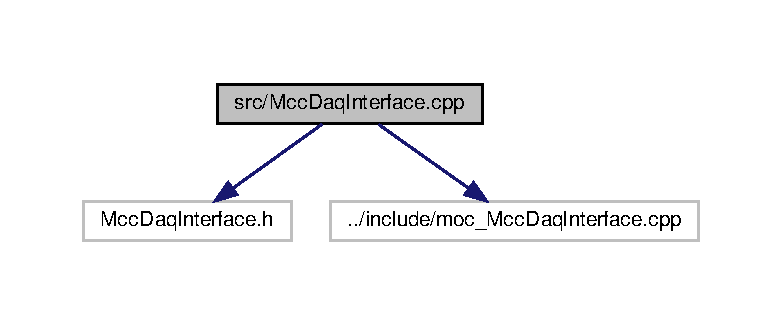
\includegraphics[width=350pt]{_mcc_daq_interface_8cpp__incl}
\end{center}
\end{figure}

\hypertarget{_mcc_daq_record_button_widget_8cpp}{}\section{src/\+Mcc\+Daq\+Record\+Button\+Widget.cpp File Reference}
\label{_mcc_daq_record_button_widget_8cpp}\index{src/\+Mcc\+Daq\+Record\+Button\+Widget.\+cpp@{src/\+Mcc\+Daq\+Record\+Button\+Widget.\+cpp}}
{\ttfamily \#include \char`\"{}Mcc\+Daq\+Record\+Button\+Widget.\+h\char`\"{}}\newline
{\ttfamily \#include \char`\"{}../include/moc\+\_\+\+Mcc\+Daq\+Record\+Button\+Widget.\+cpp\char`\"{}}\newline
Include dependency graph for Mcc\+Daq\+Record\+Button\+Widget.\+cpp\+:
\nopagebreak
\begin{figure}[H]
\begin{center}
\leavevmode
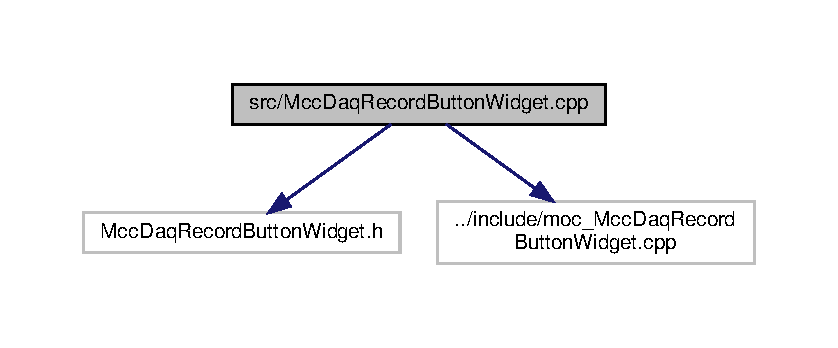
\includegraphics[width=350pt]{_mcc_daq_record_button_widget_8cpp__incl}
\end{center}
\end{figure}

\hypertarget{_mouse_interface_8cpp}{}\section{src/\+Mouse\+Interface.cpp File Reference}
\label{_mouse_interface_8cpp}\index{src/\+Mouse\+Interface.\+cpp@{src/\+Mouse\+Interface.\+cpp}}
{\ttfamily \#include \char`\"{}include/\+Mouse\+Interface.\+h\char`\"{}}\newline
{\ttfamily \#include \char`\"{}../include/moc\+\_\+\+Mouse\+Interface.\+cpp\char`\"{}}\newline
Include dependency graph for Mouse\+Interface.\+cpp\+:
\nopagebreak
\begin{figure}[H]
\begin{center}
\leavevmode
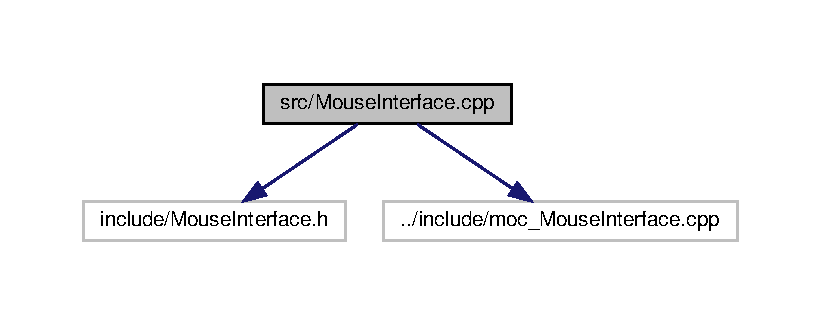
\includegraphics[width=350pt]{_mouse_interface_8cpp__incl}
\end{center}
\end{figure}

\hypertarget{_network_tab_widget_8cpp}{}\section{src/\+Network\+Tab\+Widget.cpp File Reference}
\label{_network_tab_widget_8cpp}\index{src/\+Network\+Tab\+Widget.\+cpp@{src/\+Network\+Tab\+Widget.\+cpp}}
{\ttfamily \#include \char`\"{}include/\+Network\+Tab\+Widget.\+h\char`\"{}}\newline
{\ttfamily \#include \char`\"{}../include/moc\+\_\+\+Network\+Tab\+Widget.\+cpp\char`\"{}}\newline
Include dependency graph for Network\+Tab\+Widget.\+cpp\+:
\nopagebreak
\begin{figure}[H]
\begin{center}
\leavevmode
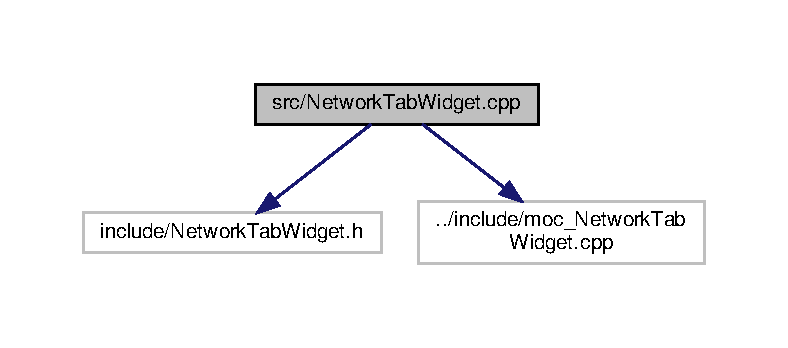
\includegraphics[width=350pt]{_network_tab_widget_8cpp__incl}
\end{center}
\end{figure}

\hypertarget{_network_tab_widget_lights_8cpp}{}\section{src/\+Network\+Tab\+Widget\+Lights.cpp File Reference}
\label{_network_tab_widget_lights_8cpp}\index{src/\+Network\+Tab\+Widget\+Lights.\+cpp@{src/\+Network\+Tab\+Widget\+Lights.\+cpp}}

\hypertarget{_parse_run_profile_8cpp}{}\section{src/\+Parse\+Run\+Profile.cpp File Reference}
\label{_parse_run_profile_8cpp}\index{src/\+Parse\+Run\+Profile.\+cpp@{src/\+Parse\+Run\+Profile.\+cpp}}
{\ttfamily \#include \char`\"{}Parse\+Run\+Profile.\+h\char`\"{}}\newline
{\ttfamily \#include \char`\"{}../include/moc\+\_\+\+Parse\+Run\+Profile.\+cpp\char`\"{}}\newline
Include dependency graph for Parse\+Run\+Profile.\+cpp\+:
\nopagebreak
\begin{figure}[H]
\begin{center}
\leavevmode
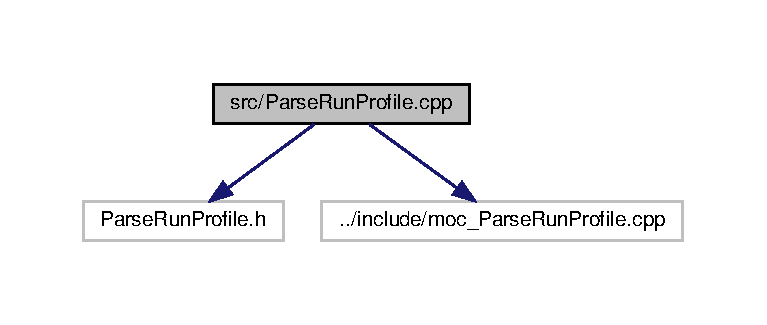
\includegraphics[width=350pt]{_parse_run_profile_8cpp__incl}
\end{center}
\end{figure}

\hypertarget{_perturbation_tab_widget_8cpp}{}\section{src/\+Perturbation\+Tab\+Widget.cpp File Reference}
\label{_perturbation_tab_widget_8cpp}\index{src/\+Perturbation\+Tab\+Widget.\+cpp@{src/\+Perturbation\+Tab\+Widget.\+cpp}}
{\ttfamily \#include \char`\"{}include/\+Perturbation\+Tab\+Widget.\+h\char`\"{}}\newline
{\ttfamily \#include \char`\"{}../include/moc\+\_\+\+Perturbation\+Tab\+Widget.\+cpp\char`\"{}}\newline
Include dependency graph for Perturbation\+Tab\+Widget.\+cpp\+:
\nopagebreak
\begin{figure}[H]
\begin{center}
\leavevmode
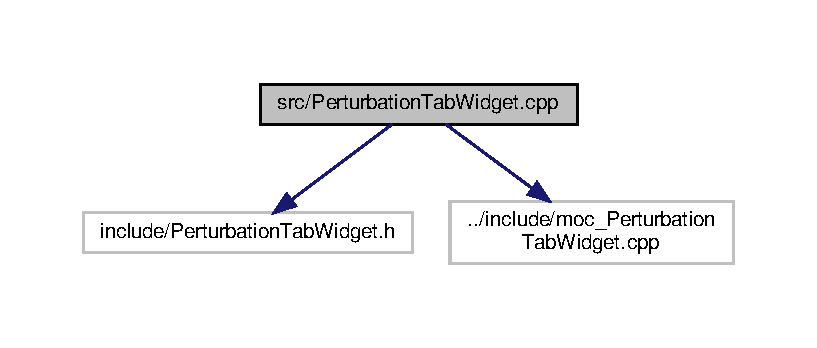
\includegraphics[width=350pt]{_perturbation_tab_widget_8cpp__incl}
\end{center}
\end{figure}

\hypertarget{_qml_interface_8cpp}{}\section{src/\+Qml\+Interface.cpp File Reference}
\label{_qml_interface_8cpp}\index{src/\+Qml\+Interface.\+cpp@{src/\+Qml\+Interface.\+cpp}}
{\ttfamily \#include \char`\"{}Qml\+Interface.\+h\char`\"{}}\newline
{\ttfamily \#include \char`\"{}../include/moc\+\_\+\+Qml\+Interface.\+cpp\char`\"{}}\newline
Include dependency graph for Qml\+Interface.\+cpp\+:
\nopagebreak
\begin{figure}[H]
\begin{center}
\leavevmode
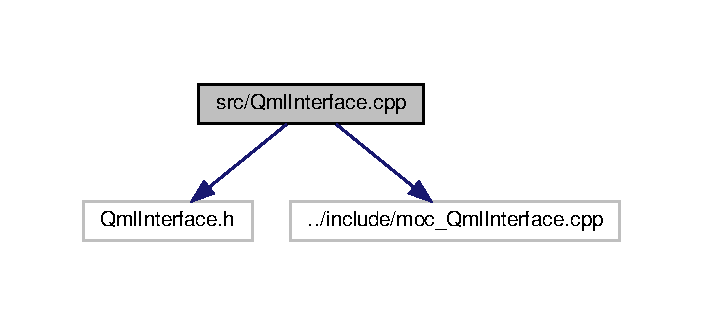
\includegraphics[width=350pt]{_qml_interface_8cpp__incl}
\end{center}
\end{figure}

\hypertarget{_read_trial_name_file_8cpp}{}\section{src/\+Read\+Trial\+Name\+File.cpp File Reference}
\label{_read_trial_name_file_8cpp}\index{src/\+Read\+Trial\+Name\+File.\+cpp@{src/\+Read\+Trial\+Name\+File.\+cpp}}
{\ttfamily \#include \char`\"{}Read\+Trial\+Name\+File.\+h\char`\"{}}\newline
Include dependency graph for Read\+Trial\+Name\+File.\+cpp\+:
\nopagebreak
\begin{figure}[H]
\begin{center}
\leavevmode
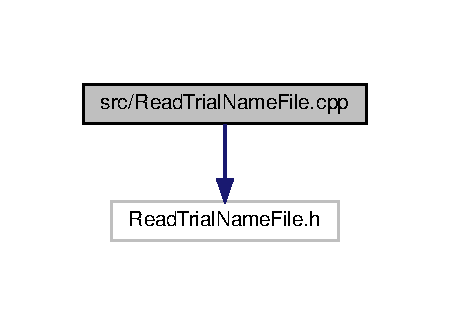
\includegraphics[width=216pt]{_read_trial_name_file_8cpp__incl}
\end{center}
\end{figure}

\hypertarget{_record_treadmill_stream_8cpp}{}\section{src/\+Record\+Treadmill\+Stream.cpp File Reference}
\label{_record_treadmill_stream_8cpp}\index{src/\+Record\+Treadmill\+Stream.\+cpp@{src/\+Record\+Treadmill\+Stream.\+cpp}}
{\ttfamily \#include \char`\"{}Record\+Treadmill\+Stream.\+h\char`\"{}}\newline
{\ttfamily \#include \char`\"{}../include/moc\+\_\+\+Record\+Treadmill\+Stream.\+cpp\char`\"{}}\newline
Include dependency graph for Record\+Treadmill\+Stream.\+cpp\+:
\nopagebreak
\begin{figure}[H]
\begin{center}
\leavevmode
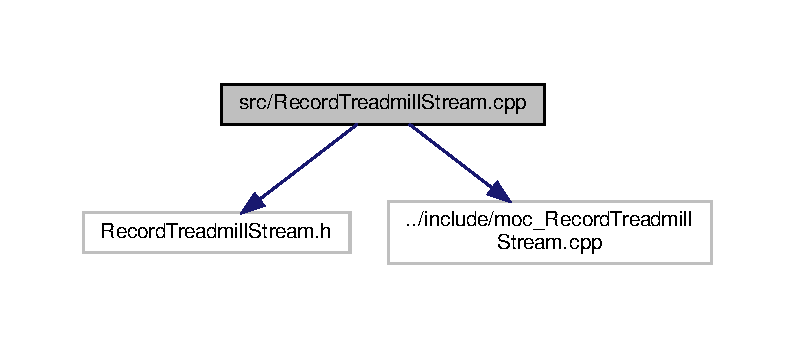
\includegraphics[width=350pt]{_record_treadmill_stream_8cpp__incl}
\end{center}
\end{figure}

\hypertarget{_send_setpoints_8cpp}{}\section{src/\+Send\+Setpoints.cpp File Reference}
\label{_send_setpoints_8cpp}\index{src/\+Send\+Setpoints.\+cpp@{src/\+Send\+Setpoints.\+cpp}}
{\ttfamily \#include \char`\"{}include/\+Send\+Setpoints.\+h\char`\"{}}\newline
Include dependency graph for Send\+Setpoints.\+cpp\+:
\nopagebreak
\begin{figure}[H]
\begin{center}
\leavevmode
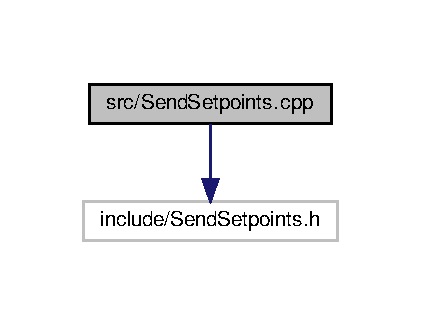
\includegraphics[width=350pt]{_send_setpoints_8cpp__incl}
\end{center}
\end{figure}

\hypertarget{_stimulator_interface_8cpp}{}\section{src/\+Stimulator\+Interface.cpp File Reference}
\label{_stimulator_interface_8cpp}\index{src/\+Stimulator\+Interface.\+cpp@{src/\+Stimulator\+Interface.\+cpp}}
{\ttfamily \#include \char`\"{}Stimulator\+Interface.\+h\char`\"{}}\newline
Include dependency graph for Stimulator\+Interface.\+cpp\+:
\nopagebreak
\begin{figure}[H]
\begin{center}
\leavevmode
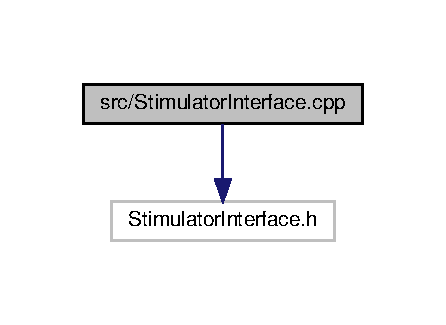
\includegraphics[width=214pt]{_stimulator_interface_8cpp__incl}
\end{center}
\end{figure}

\hypertarget{_subject_interface_8cpp}{}\section{src/\+Subject\+Interface.cpp File Reference}
\label{_subject_interface_8cpp}\index{src/\+Subject\+Interface.\+cpp@{src/\+Subject\+Interface.\+cpp}}
{\ttfamily \#include \char`\"{}../include/\+Subject\+Interface.\+h\char`\"{}}\newline
{\ttfamily \#include \char`\"{}../include/moc\+\_\+\+Subject\+Interface.\+cpp\char`\"{}}\newline
Include dependency graph for Subject\+Interface.\+cpp\+:
\nopagebreak
\begin{figure}[H]
\begin{center}
\leavevmode
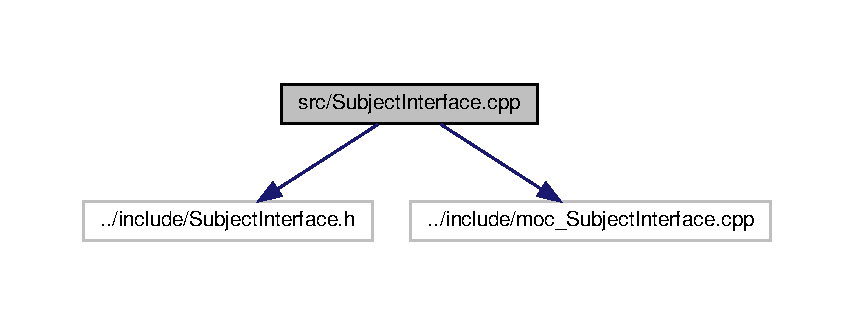
\includegraphics[width=350pt]{_subject_interface_8cpp__incl}
\end{center}
\end{figure}

\hypertarget{_subject_interface_widget_8cpp}{}\section{src/\+Subject\+Interface\+Widget.cpp File Reference}
\label{_subject_interface_widget_8cpp}\index{src/\+Subject\+Interface\+Widget.\+cpp@{src/\+Subject\+Interface\+Widget.\+cpp}}
{\ttfamily \#include \char`\"{}Subject\+Interface\+Widget.\+h\char`\"{}}\newline
{\ttfamily \#include \char`\"{}../include/moc\+\_\+\+Subject\+Interface\+Widget.\+cpp\char`\"{}}\newline
Include dependency graph for Subject\+Interface\+Widget.\+cpp\+:
\nopagebreak
\begin{figure}[H]
\begin{center}
\leavevmode
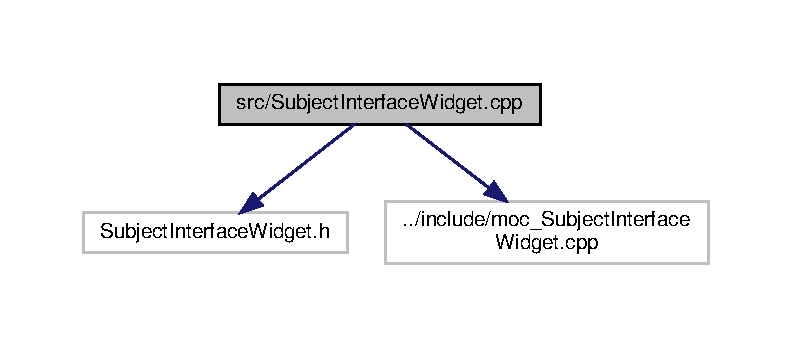
\includegraphics[width=350pt]{_subject_interface_widget_8cpp__incl}
\end{center}
\end{figure}

\hypertarget{_treadmill_automation_8cpp}{}\section{src/\+Treadmill\+Automation.cpp File Reference}
\label{_treadmill_automation_8cpp}\index{src/\+Treadmill\+Automation.\+cpp@{src/\+Treadmill\+Automation.\+cpp}}
{\ttfamily \#include \char`\"{}include/\+Treadmill\+Automation.\+h\char`\"{}}\newline
{\ttfamily \#include \char`\"{}../include/moc\+\_\+\+Treadmill\+Automation.\+cpp\char`\"{}}\newline
Include dependency graph for Treadmill\+Automation.\+cpp\+:
\nopagebreak
\begin{figure}[H]
\begin{center}
\leavevmode
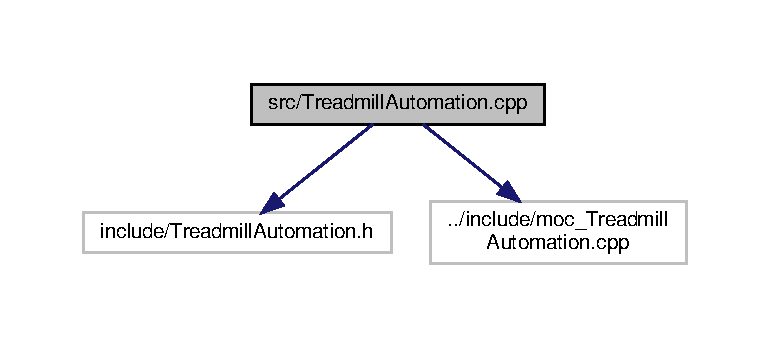
\includegraphics[width=350pt]{_treadmill_automation_8cpp__incl}
\end{center}
\end{figure}

\hypertarget{_treadmill_automation_db_i_face_8cpp}{}\section{src/\+Treadmill\+Automation\+Db\+I\+Face.cpp File Reference}
\label{_treadmill_automation_db_i_face_8cpp}\index{src/\+Treadmill\+Automation\+Db\+I\+Face.\+cpp@{src/\+Treadmill\+Automation\+Db\+I\+Face.\+cpp}}
{\ttfamily \#include \char`\"{}Treadmill\+Automation\+Db\+I\+Face.\+h\char`\"{}}\newline
{\ttfamily \#include \char`\"{}../include/moc\+\_\+\+Treadmill\+Automation\+Db\+I\+Face.\+cpp\char`\"{}}\newline
Include dependency graph for Treadmill\+Automation\+Db\+I\+Face.\+cpp\+:
\nopagebreak
\begin{figure}[H]
\begin{center}
\leavevmode
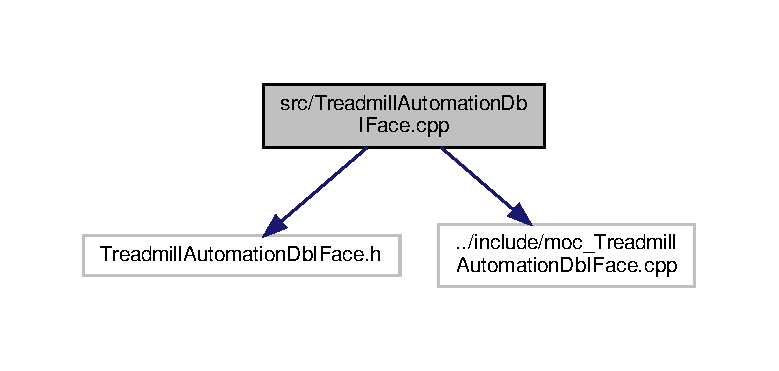
\includegraphics[width=350pt]{_treadmill_automation_db_i_face_8cpp__incl}
\end{center}
\end{figure}

%--- End generated contents ---

% Index
\backmatter
\newpage
\phantomsection
\clearemptydoublepage
\addcontentsline{toc}{chapter}{Index}
\printindex

\end{document}
